% Dibentuk oleh kkciv_vintage.h15.render dari results/processed/h15-figure-data.csv.
% Jangan disunting langsung; jalankan make h15-figures untuk membentuk ulang.
\documentclass[border=2pt]{standalone}
\usepackage[T1]{fontenc}
\usepackage{pgfplots}
\pgfplotsset{compat=1.18}
\pgfplotsset{/pgf/number format/.cd, use comma, 1000 sep={.}}
\usepgfplotslibrary{groupplots}
\ifdefined\pdfvariable
  \pdfvariable suppressoptionalinfo \numexpr 1+2+4+8+16+32+64+128+256+512\relax
\fi

\begin{document}
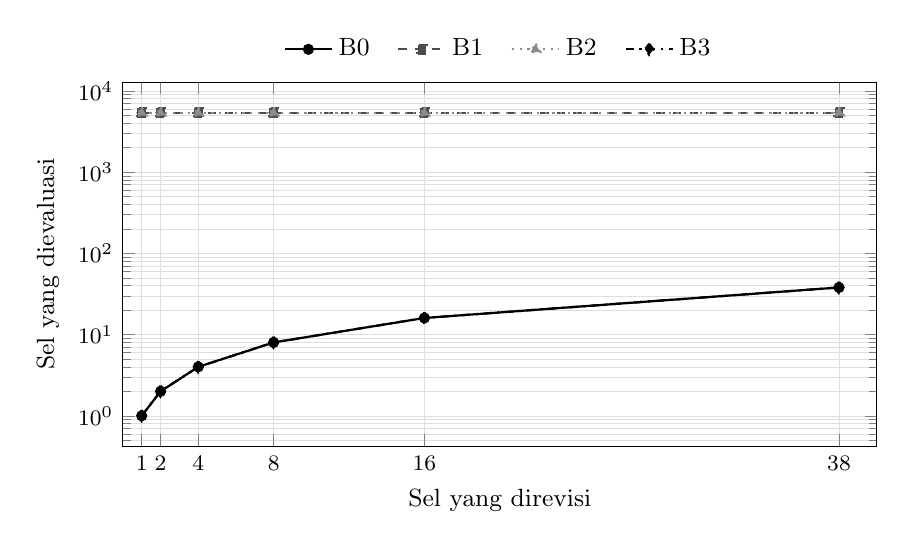
\begin{tikzpicture}
\begin{axis}[
  xlabel={Sel yang direvisi},
  ylabel={Sel yang dievaluasi},
  xtick={1,2,4,8,16,38},
  xmin=0, xmax=40,
  width=0.92\linewidth, height=6.2cm,
  legend style={font=\small, at={(0.5,1.03)}, anchor=south, legend columns=4, draw=none, /tikz/every even column/.append style={column sep=8pt}},
  grid=both, grid style={line width=0.2pt, draw=gray!25},
  tick label style={font=\footnotesize}, label style={font=\small},
  ymode=log,
]
\addplot[mark=*, mark size=1.6pt, color=black, thick, error bars/.cd,
  y dir=both, y explicit]
table[row sep=\\, y error plus index=2, y error minus index=3] {
x y eplus eminus \\
1 1 0.000000 0.000000 \\
2 2 0.000000 0.000000 \\
4 4 0.000000 0.000000 \\
8 8 0.000000 0.000000 \\
16 16 0.000000 0.000000 \\
38 38 0.000000 0.000000 \\
};
\addlegendentry{B0}
\addplot[mark=square*, mark size=1.6pt, color=black!70, thick, dashed, error bars/.cd,
  y dir=both, y explicit]
table[row sep=\\, y error plus index=2, y error minus index=3] {
x y eplus eminus \\
1 5378 0.000000 0.000000 \\
2 5378 0.000000 0.000000 \\
4 5378 0.000000 0.000000 \\
8 5378 0.000000 0.000000 \\
16 5378 0.000000 0.000000 \\
38 5378 0.000000 0.000000 \\
};
\addlegendentry{B1}
\addplot[mark=triangle*, mark size=2pt, color=black!45, thick, dotted, error bars/.cd,
  y dir=both, y explicit]
table[row sep=\\, y error plus index=2, y error minus index=3] {
x y eplus eminus \\
1 5378 0.000000 0.000000 \\
2 5378 0.000000 0.000000 \\
4 5378 0.000000 0.000000 \\
8 5378 0.000000 0.000000 \\
16 5378 0.000000 0.000000 \\
38 5378 0.000000 0.000000 \\
};
\addlegendentry{B2}
\addplot[mark=diamond*, mark size=2pt, color=black, thick, dashdotted, error bars/.cd,
  y dir=both, y explicit]
table[row sep=\\, y error plus index=2, y error minus index=3] {
x y eplus eminus \\
1 1 0.000000 0.000000 \\
2 2 0.000000 0.000000 \\
4 4 0.000000 0.000000 \\
8 8 0.000000 0.000000 \\
16 16 0.000000 0.000000 \\
38 38 0.000000 0.000000 \\
};
\addlegendentry{B3}
\end{axis}
\end{tikzpicture}
\end{document}
